\newpage
\section{Общие настройки системы}

Система администрирования ЛПУ (или система) работает через Web-интерфейс и не требует установки на клиентской рабочей станции никакого дополнительного программного обеспечения. Единственным обязательным условием является наличие установленного Web-браузера, который, как правило, включен по умолчанию при установке любой операционной системы.

Вся работа в системе производится в окне Web-браузера. В верхней части каждой страницы находится панель управления (Рисунок \ref{img_gen_main}).

\begin{figure}[ht]\centering
 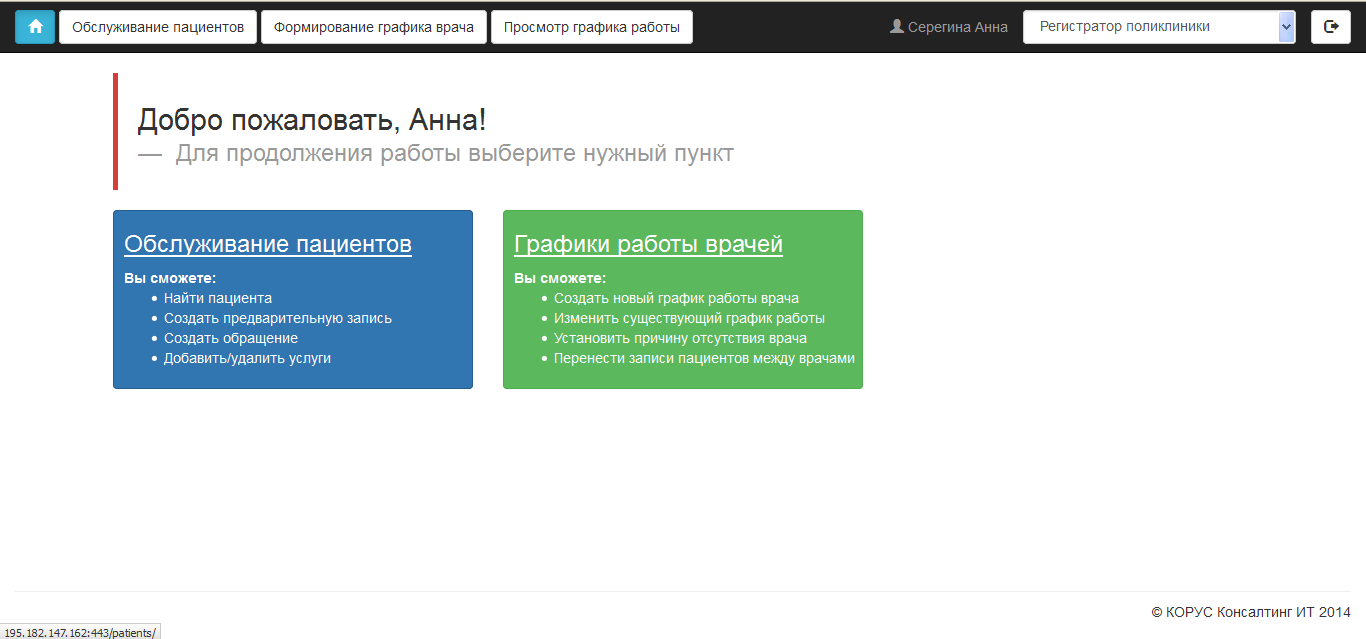
\includegraphics[width = 1\textwidth ,keepaspectratio]{gen_main}
 \caption{Главная страница системы}
 \label{img_gen_main}
\end{figure} 

В левой ее части находятся список доступных подсистем. При нажатии на кнопку с названием подсистемы осуществляется переход на главную страницу выбранной подсистемы. При нажатии на кнопку 
\includegraphics{home} выполняется переход на главную страницу системы.

В правой части панели управления находятся следующие кнопки:
\begin{itemize}
 \item Кнопка 
\includegraphics{help}  вызывает справку по основным управляющим элементам текущей страницы.
 \item Кнопка  
\includegraphics{user} позволяет перейти на страницу управления доступом пользователей.
 \item Кнопка  
\includegraphics{conf} осуществляет переход к настройкам, общим для всей системы.
 \item Кнопка 
\includegraphics{exit}  позволяет выйти из системы.
\end{itemize}
 
\subsection{Управление доступом пользователей}

Для перехода на страницу управления доступом пользователей следует на любой странице системы нажать кнопку 
\includegraphics{user} верхней панели. Откроется страница, содержащая список пользователей системы (Рисунок \ref{img_gen_users}).

\begin{figure}[ht]\centering
 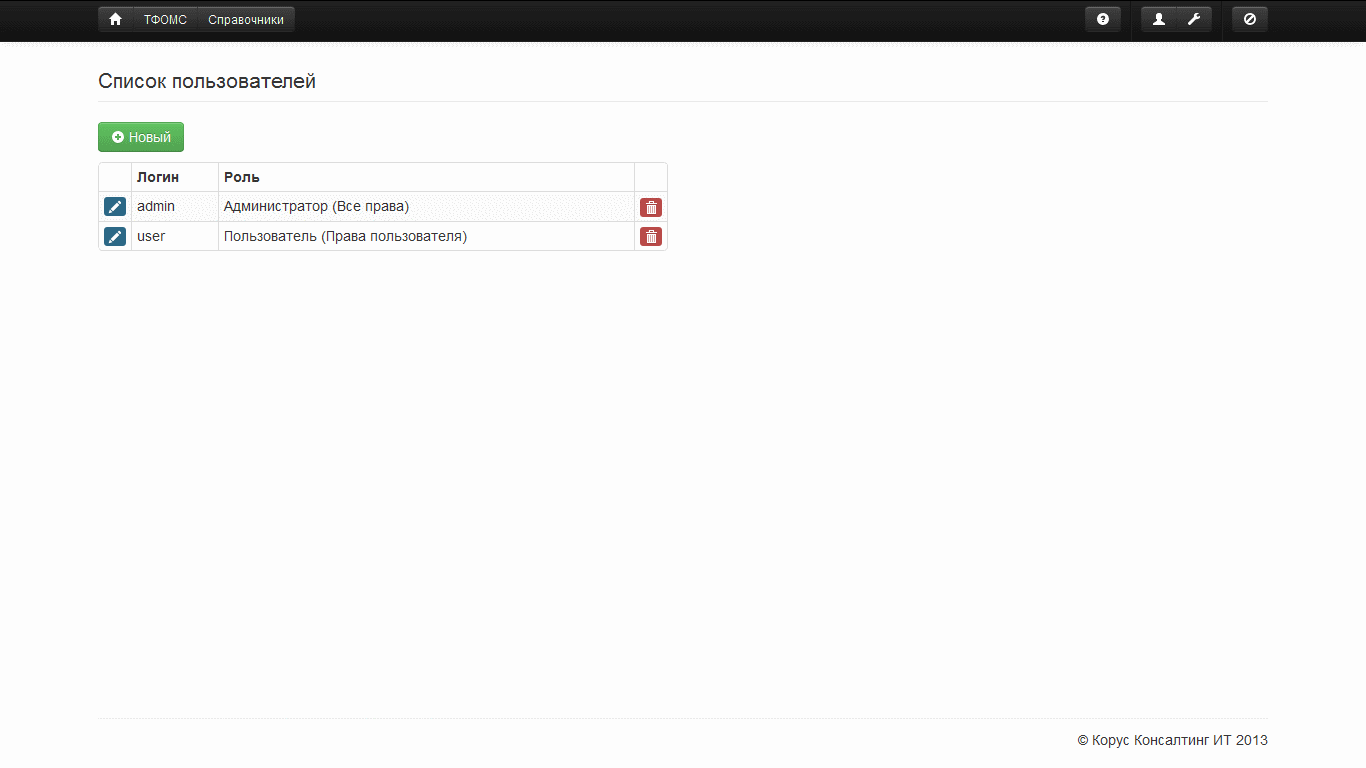
\includegraphics[width = 1\textwidth ,keepaspectratio]{gen_users}
 \caption{Страница управления доступом пользователей}
 \label{img_gen_users}
\end{figure} 

Для добавления нового пользователя нужно нажать кнопку \btn{Новый}  в верхней части страницы. Откроется новая страница, где необходимо ввести уникальный идентификатор пользователя (\dm{Логин}), дважды ввести пароль, который пользователь будет использовать для входа в систему (значения полей \dm{Пароль} и \dm{Повторите пароль} должны совпадать), и выбрать роль пользователя в системе. После того, как все поля будут заполнены, нужно нажать кнопку \btn{Сохранить}. Новый пользователь будет добавлен в список.

\begin{figure}[ht]\centering
 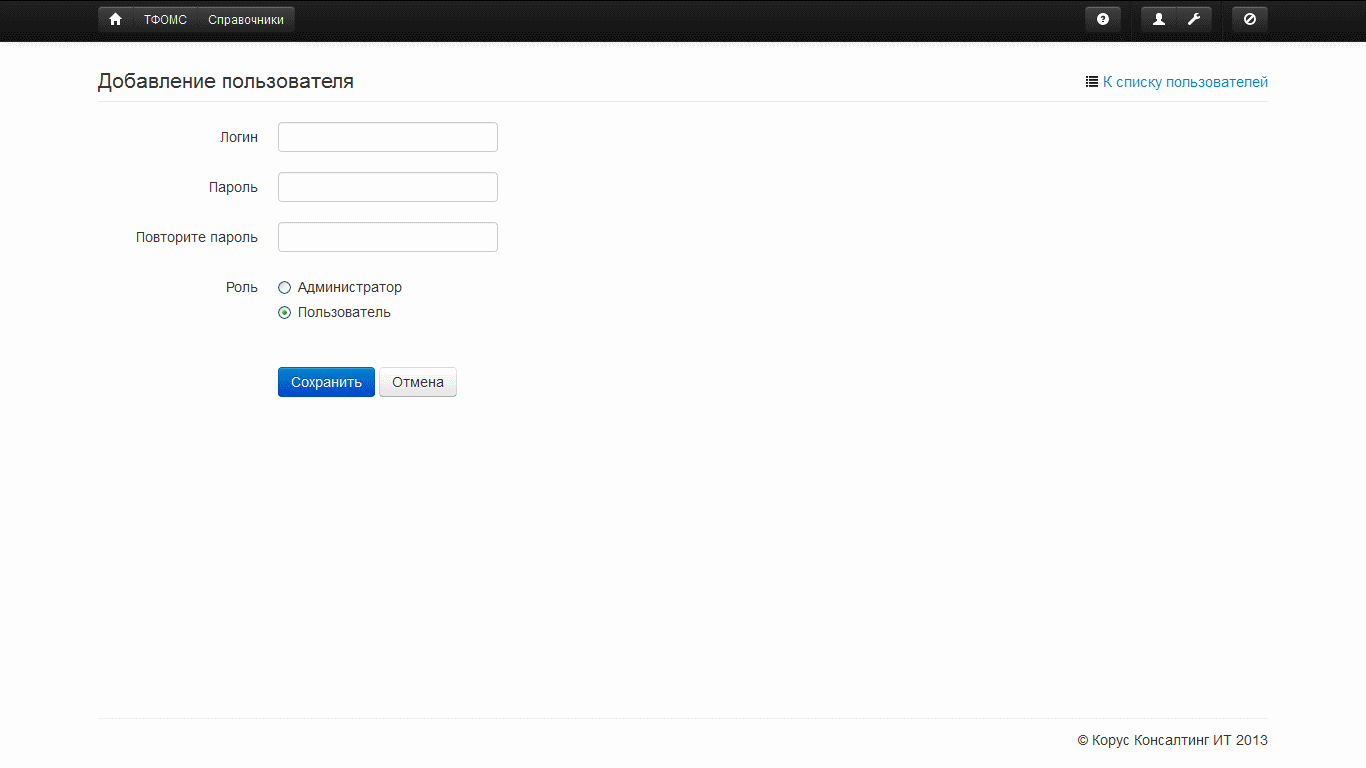
\includegraphics[width = 1\textwidth ,keepaspectratio]{gen_user_add}
 \caption{Страница редактирования профиля пользователя}
 \label{img_gen_user_add}
\end{figure}

Для редактирования данных пользователя следует нажать кнопку 
\includegraphics{edit} , слева от соответствующей записи в списке пользователей. Откроется страница редактирования данных пользователя (Рисунок \ref{img_gen_user_add}). После изменения данных их необходимо сохранить, нажав кнопку \btn{Сохранить}.

Для удаления пользователя из системы нужно нажать кнопку 
\includegraphics{del}. Появится диалоговое окно, где необходимо подтвердить удаление, после чего пользователь будет удален из системы и из списка пользователей соответственно.

\subsection{Глобальные настройки системы} \label{gen_conf}

Для перехода на страницу общих настроек системы следует на любой странице системы нажать кнопку 
\includegraphics{conf}  верхней панели. Откроется страница, содержащая настройки системы (Рисунок 4).

\begin{figure}[ht]\centering
 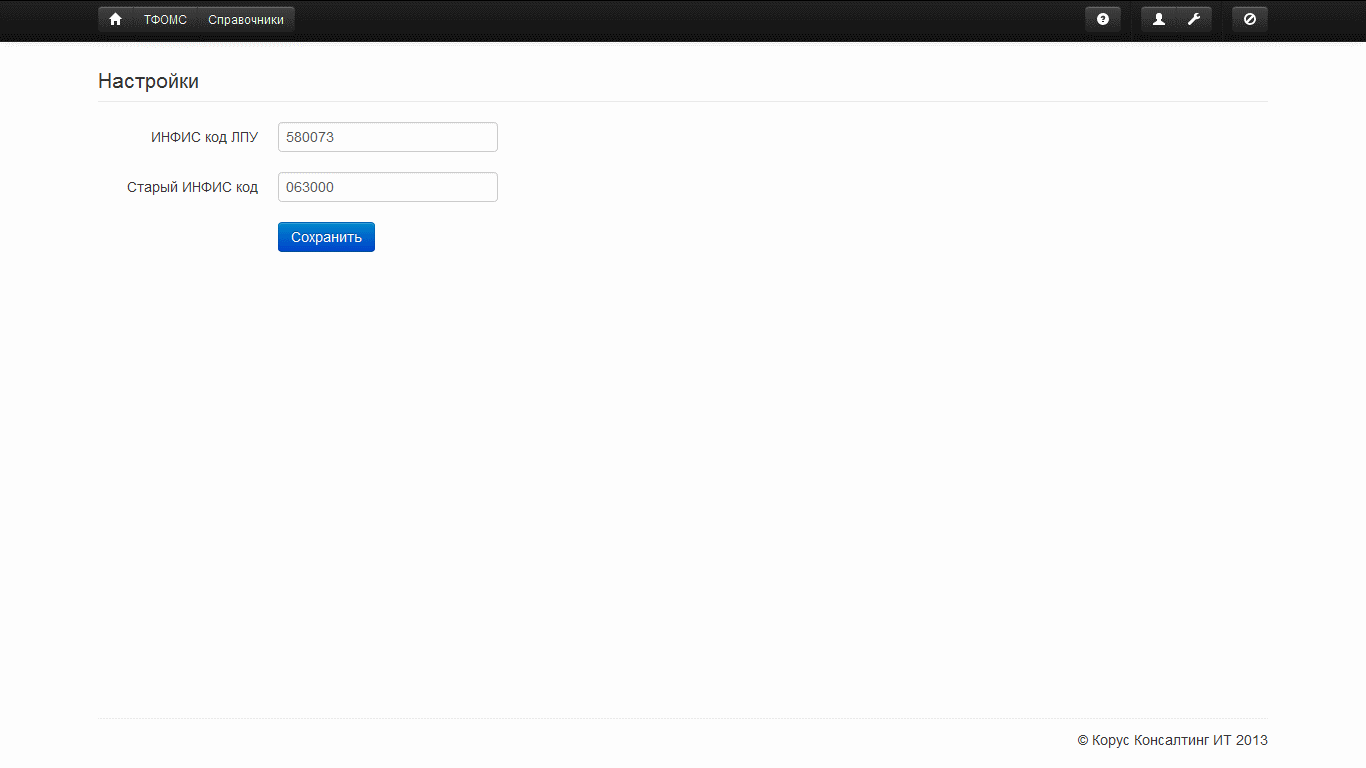
\includegraphics[width = 1\textwidth ,keepaspectratio]{gen_conf}
 \caption{Общие настройки системы}
 \label{img_gen_conf}
\end{figure}

Настройки содержат следующие параметры:
\begin{itemize}
 \item \dm{ИНФИС код ЛПУ} – данный код используется в качестве внешнего кода ЛПУ в различных выгрузках и при взаимодействии с внешними системами.
 \item \dm{Старый ИНФИС код} – старый код.
\end{itemize}
 
После изменения настроек следует нажать кнопку \btn{Сохранить}.
